\documentclass[10pt,a4paper]{article}
\usepackage[utf8]{inputenc}
\usepackage[english]{babel}
\usepackage{amsmath}
\usepackage{amsfonts}
\usepackage{amssymb}
\usepackage{graphicx}
\usepackage{verbatim}
\usepackage{listings}
%\usepackage[left=2cm,right=2cm,top=2cm,bottom=2cm]{geometry}
\usepackage{makeidx}
\usepackage{fancyhdr}
\pagestyle{fancy}
\usepackage{lastpage}
\usepackage{indentfirst}

\begin{document}

\lhead{
\includegraphics[width=1cm]{feup_logo.png}}
\chead{}
\rhead{Faculty of Engineering of Porto's University}

\lfoot{AIAD}
\cfoot{ Traffic Lights Management by Reinforcement Multi-Agent System }
\rfoot{ \thepage\ of \pageref{LastPage}}

\begin{titlepage}
    \centering
    {\bfseries\Large
        Traffic Lights Management by Distributed Cooperation-Based System\\   
    }
    \vfill
    \vfill
	
\includegraphics[width=5cm]{feup_logo.png}\\
	Faculty of Engineering of Porto's University
    \vfill
    \vfill
    \centering
     Diogo Pinto      ei11120\\
     João Santos      ei11126\\
     Rui Batista      ei06013\\
    \vfill
   {\bfseries\Large  Agents and Distributed Artificial Intelligence\\
   }
    \vfill
    \vfill
    \vfill
\end{titlepage}

\newpage

\tableofcontents
\newpage

\begin{abstract}

\end{abstract}
The need to transport people and goods obligate human species on relying in travel through predetermined pathways. But one evolution wall encountered are traffic jams, which reduce even furder the speed at wish the transportations are made. This lead to the research of numerous ways to improve this situation, being one of the most prominent the development of intelligent intersections organizers, namely traffic lights.

\newpage

\section{Introduction}

\subsection{Context}

    	With the advance of civilization, the population level is arising and with that the number of vehicles is coming to an alarming number. One of the most popular options to deal with it, is the creation of roundabouts and crossings, but those are reveling to be a bigger problem than the initial one, creating big jams and slowing the traffic even more. To solve this problem traffic lights have been created, these have the ability of splitting traffic and moderate it, so it can flow better creating lesser delays. 

	The traffic lights work by allowing different lanes to cross in a phased way so creating a constant traffic flow. These phases normally are fixed, for example, the green phase duration is always  50 seconds, there are some variations, when a person presses the cross walk button to pass, there is a mechanism that alters the normal behavior of the traffic light and turns every other phase into a red phase so the person can pass safely, it's a kind of subsuption mechanism.


\subsection{Objectives}
	Although there are many different ways to work with traffic lights, it is proposed the testing and validation of a multi-agent system, establishing the parallel with the existing methods (fixed/subsuption). This system will bear in mind that the behavior of one traffic light can influence both direct and indirect neighbors. The focus of this project is, then, to improve the global traffic patterns, paying attention for special vehicles, such as emergency and public transports.
   
	To analyze which solution is better, as well as the significance of the improvement, we have to compare them in terms of performance. For that we are going to measure:
\begin{itemize}
\item waiting time in cue 
\item average speed in the network
\item average speed of public transports in the network
\item average speed of emergency vehicles
\end{itemize}
	These metrics are going to be taken on different times of day, resulting on three levels of traffic, ranging from sub-saturated to over-saturates.
    
  	Then, the traffic lights strategies to be measured are as follows:
\begin{itemize}
\item fixed-time
\item greedy
\item cooperating
\end{itemize}

\newpage

\section{Platforms/Tools}
\subsection{Jade}
	Jade (Java Agent Development Network) is a FIPA-compliant framework for simplifying  the development of multi-agent systems written in Java. It accomplishes this through middle-ware in conformity with FIPA specifications and a set of graphical tools to help with development and debugging. Another facility is that it can be distributed across multiple machines (which may or may not share the same OS) transparently to the end user. Configurations may be altered in run-time like moving agents from one machine to another.
    
    Besides the agent abstraction, JADE provides a task execution and composition model, peer to peer agent communication based on asynchronous messages, a yellow pages service supporting publish subscribe discovery mechanism and many other features that facilitate the development of a distributed system.
    
    Additionally the platform has the possibility of executing the behavior of agents in parallel, as well as support for the definition of languages and ontologies. 
    
\begin{center}
    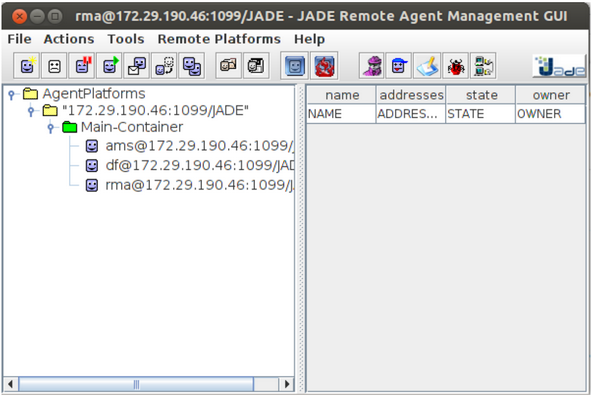
\includegraphics[width=1.0\textwidth]{Capture.PNG}
    \textbf{Figure 1:} JADE GUI
\end{center}

\subsection{TraSMAPI}
	TraSMAPI is a generic API that allows real-time communication between agents and an urban traffic environment created by various simulators. This tool was developed in LIACC (Artificial Intelligence and Computer Science Laboratory), in the University of Porto, and has already been tested with two different urban traffic scenario simulators, including SUMO. In our case we will be using it in conjunction with JADE and SUMO.
	
    This API offers a high abstraction level such that the solution is independent from the microscopic simulator.
    
\begin{center}
    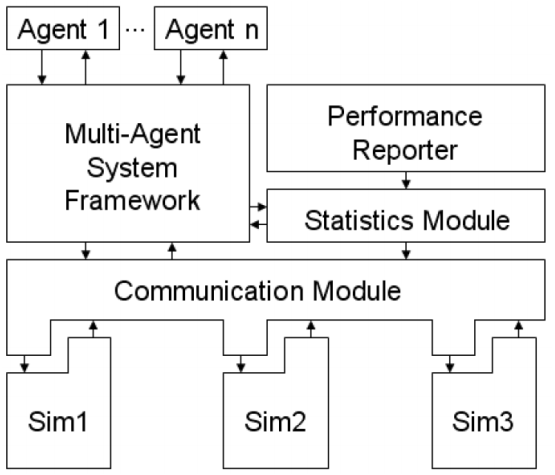
\includegraphics[width=0.5\textwidth]{trasmapi.PNG} \\
    \textbf{Figure 2:} TranSMAPI architecture
\end{center}
    
    There are three main modules as seen in the figure above: the communication module, the statistic generation module and the MAS management module. We will only be using the communications module.

\subsection{SUMO}
	SUMO (Simulation of Urban MObility) is a tool to simulate microscopic and continuous traffic patterns. The simulation model is microscopic, meaning each vehicle is independent and modeled explicitly. It was developed to emulate and study the traffic of large cities, but can be used to simulate small intersections, which is enough for our experiment. 
    
    SUMO can model different vehicle types, multi-lane roads, traffic lights, crossroads and many other types of road networks. 
    
    SUMO has a graphical interface so users can visualize the network and entities being modeled as the simulation progresses.     
    
\begin{center}
    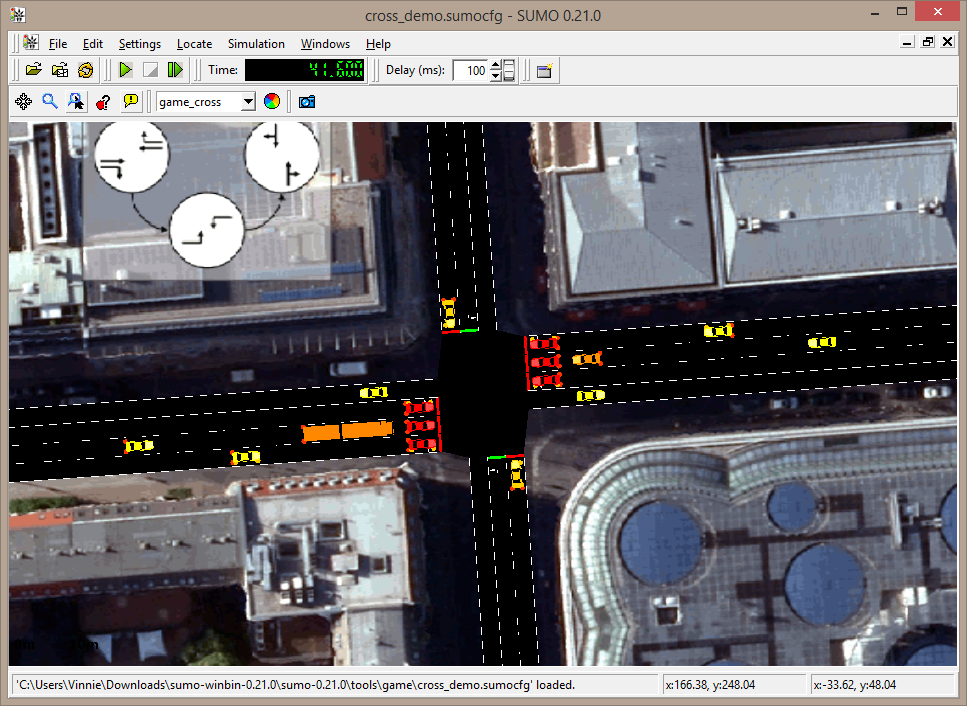
\includegraphics[width=1.0\textwidth]{sumo.PNG}
    \textbf{Figure 3:} SUMO example intersection
\end{center}    
    
    SUMO also allows inter-operability with other applications in real-time through an API called TraCI. This allows us to change traffic light states using an external agent management framework such as JADE.
    
    It is also possible to load different maps quickly into SUMO. The maps are described using XML files. This makes the task of testing with different scenarios faster and easier.
   
\subsection{Tool-chain}
    
\begin{center}
    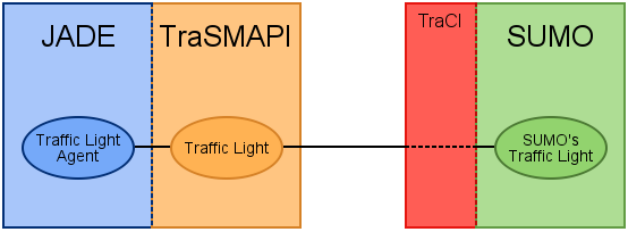
\includegraphics[width=1.0\textwidth]{toolchain.PNG}
    \textbf{Figure 4:} Application tools communication channels
\end{center}

	The figure above represents the architecture that will be used to conduct our simulations during this experiment. This architecture makes it possible to simulate one or more traffic light agents. Each agent will have its own representation in SUMO and the communication between them will be handle by TraSMAPI.
\newpage

\section{Specification}

\subsection{Agents Architecture}
	Due to the nature of the problem, it is best modeled as a \textit{swarm-intelligence} problem, giving a high degree of individuality and communication to each of the intervening elements relative to the other ones. By other words, each traffic light will not only pursue individually its own objectives, but also have a behavior that will determine how it will change state to reach those goals, always learning from experience. In that sense, this fits the definition of a \textbf{adaptative \textit{computational agent}}.\cite{Chin2013} 
    
\subsubsection{Agents PAGE Description}
    That agent is described, according to the PAGE agent's description as follows
    
    \begin{itemize}
    \item Perceptions
        \begin{itemize}
        \item time of the day
        \item amount of traffic retained by it
        \item existence of any priority vehicle
        \item existence of any public vehicle
        \end{itemize}
        
    \item Actions
        \begin{itemize}
        \item increase the green-light time
        \item decrease the green-light time
        \item warn neighbors about potential approximation of emergency vehicles \\
        	(conveyed in messages to other agents)
        \item ask permission to change to green \\
        	(conveyed in messages to other agents)
        \end{itemize}
        
    \item Goals
        \begin{itemize}
        \item minimize vehicles in queue
        \item minimize green-time in cycle \\
        	by minimizing the green-light time we enable lower red-light same-intersection traffic lights of a single cycle
        \end{itemize}
        
    \item Environment
        \begin{itemize}
        \item roads with intersections
        \end{itemize}
    \end{itemize}

\subsubsection{Agents Properties}
    
    \textbf{Internal:}
    \begin{itemize}
    \item \textbf{Lifetime:} permanent
    \item \textbf{Cognition level:} balanced between reactive and functional
    \item \textbf{Implementation:} procedural
    \item \textbf{Mobility:} static
    \item \textbf{Adaptability:} self-learner 
    \end{itemize}

	\textbf{External:}
    \begin{itemize}
    \item \textbf{Location:} local
    \item \textbf{Social autonomy:} mostly independent \\
    	the agent is lightly controlled by others in the sense of taking the advice of neighbors about the approximation of emergency vehicles
    \item \textbf{Sociability:} member
    \item \textbf{Collaboration:} cooperative
    \item \textbf{Interaction:} agent-agent
    \end{itemize}
    
    \textbf{Multi-Agents System:}
    \begin{itemize}
    \item \textbf{Uniformity:} homogeneous
    \item \textbf{Granularity:} fine-grained
    \item \textbf{Control:} decentralized
    \end{itemize}

\subsection{Learning Algorithms}
	The problem of coordinating traffic lights has seen solutions (with their respective pros and cons) through many algorithms. 
    
    As the main interest on this problem is to improve by learning, one of the first options is \textit{neural networks}. Although its initial appeal, it requires a training set very large. On the other hand, \textit{fuzzy logic}, which can effectively translate the linguistic values of the problem into numerical, treatable ones. But this one also has a big flaw: it does not learn. Another option would be a \textit{genetic algorithm}, if were not the case of being too expensive to keep up with the dynamic changes of traffic flow. \cite{Oliveira2006} 
    
    Exhausting all the options, the one category of algorithms most fit is \textit{reinforcement learning} algorithms. With this algorithms, the agents agents.start off with an inefficient state, and improve itself as it acquires experiences. From this category, \textit{Q-Learning} protrudes by, in each decision time, taking into account not only the actions (that is, the status arrived by it), but also the states caused by the actions.

\subsubsection{Q-Learning}
	Q-Learning is a reinforcement learning algorithm, which bases its decisions on the best \textbf{Q Quality} for a given current state and action. After a sufficient number of experiences, the algorithm converges to a maximum, in respect to the best combination of state-actions. \cite{acetatos2014}
    
    This is achieved through the evaluation of a \textit{reinforcement function}, which derives from the agent's objectives. Alongside this, the \textit{value functions} determine how good is to take an action in a given state.
\\
\\
    $Q(s, a) = Q(s, a) + \alpha [r + \gamma max_{a'} Q(s', a') - Q(s, a)]$, \\
    where $0 <= \alpha <= 1$ is the learning rate, \\
    $r$ is the reinforcement obtained by executing action $a$ on state $s$ \\
    


\subsection{Problem's Design Decisions}

\begin{itemize}
\item	Each traffic light will have a fixed phase sequence. Each one has a time frame and color (which corresponds to a driver's behavior), namely green, yellow and red.
    
\item 	The queues ahead of each traffic light will be categorized to one of four orders of magnitude, ranging from no traffic to high volume of traffic.
    
\item	The states of the traffic lights will be susceptible to invariants, to keep a logical behavior on the system. This will keep the vehicles behind the intersection and not waiting in the middle of it.
    
\begin{center}
    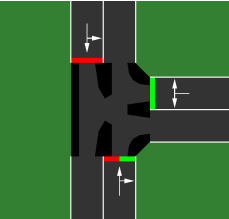
\includegraphics[width=0.5 \textwidth]{snapshot3.png} \\
    \textbf{Figure 5:} Basic intersection
\end{center}

	To illustrate this, the \textit{Figure 5} represents an invalid state, where for the vehicles coming from the right will encounter inside the intersection cars coming from bellow.


\end{itemize}
\newpage

\subsection{Project's Development Stages}

	At this stage the team has gained a strong foundations with the concepts, algorithms and tools, as well as agreed on the main design decisions, feeling very capable of starting developing the application itself.
    
    The first few weeks will be assigned to develop the core application, with support for regular traffic, and agents with \textit{fixed-time}, \textit{greedy} and \textit{cooperating} approaches.
    
    Following after, tests and measures will be made, in order to retrieve the main conclusions for the project.
    
    In the last stage, it will be implemented a mode with emergency vehicles and public transports, which will have its own tests and measures phase.

\newpage

\section{Resources}
\subsection{Bibliography}
\bibliography{biblio}
\bibliographystyle{acm}

\end{document}